
\chapter{Notions et préliminaire}
\begin{minipage}{\textwidth}
	\linespread{1.2}
	\minitoc
\end{minipage}

\section{Les réseaux complexes}

\subsection{Introduction}
 La recherche sur les réseaux complexes peut être conceptualisée comme se situant à l'intersection entre la théorie 
 des graphes et la mécanique statistique, ce qui lui confère une nature multidisciplinaire. Alors que 
 son origine remonte aux travaux pionniers sur la percolation et les graphes aléatoires de Flory \cite{Flory} et  Erd\H{o}s-Rényi \cite{Erdos-Renyi1959,Erdos-Renyi1960,Erdos-Renyi1961}, la recherche dans les réseaux complexes n'est 
 devenue une priorité que récemment. La principale raison  est la découverte que les réseaux réels ont des caractéristiques 
 qui ne sont pas expliquées par une connectivité aléatoire uniformément distribuée. En effet, les réseaux  
 réelles posèdent  des distributions de degré en loi de puissance et des hubs, parmi d'autres caractéristiques 
 structurelles. Trois développements particuliers ont fortement contribué aux 
 développements en cours: l'étude de Watts et Strogatz sur les réseaux petit monde \cite{WS1998}, la caractérisation par
 Barab\'{a}si-Albert (BA) des modèles sans échelle  \cite{BA1999}, et l'identification par Girvan et Newman des structures communautaires 
 présentes dans de nombreux réseaux \cite{Girvan}.
 \subsection{Définition}
  Un \textsf{réseau} est une collection de points réunis sous forme de paires, les points sont appelés nœuds ou sommets 
  et les lignes sont appelées liens ou arêtes. Le mot \textsf{complexe} est en général le résultat de  l'évolution 
  décentralisée et non planifiée dans ces réseaux (Fig.~\ref{exemples-reseaux}). De nombreux objets d'intérêt dans
  les sciences physiques, informatiques, biologiques et sociales peuvent être considérés comme des réseaux complexes. 
  Un réseau en général est une représentation simplifiée  qui réduit un système à une structure abstraite capturant 
  uniquement les bases des modèles de connexion, les nœuds  et les liens peuvent être accompagnés
  d'informations supplémentaires pour capturer plus de détails du système. 
  %Même s'il y a un inconvénient de 
  %perte d'informations dans le processus de réduction d'un système complet
  %à une représentation par réseau, il présente également de grands avantages
  
  \begin{figure}[h!]
  	\centering
  	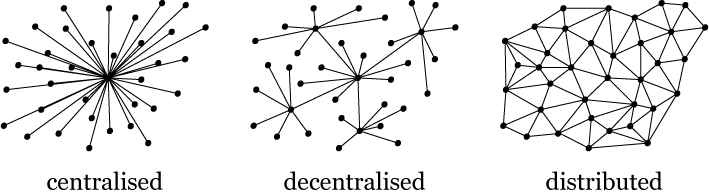
\includegraphics[scale=0.55]{./figures/types-networks2}
  	\caption{Représentation de quelques types de réseaux composés par des nœuds et des liens. }
  	\label{exemples-reseaux}
  \end{figure}
 \subsection{Différents types des Réseaux complexes}
  L'étude des réseaux complexes a été inspirée par le désir de comprendre les différents systèmes réels, allant 
  des réseaux de communications aux réseaux écologiques. Les bases de données empiriques disponibles pour l'étude
  couvrent plusieurs disciplines, en générale, elles se divisent en quatre grandes catégories: Réseaux Technologiques,
  Réseaux Biologiques, Réseaux Sociaux et Réseaux d'Informations.
 \subsubsection{Réseaux Technologiques}
  Les réseaux technologiques sont des réseaux artificiels, qui ont grandi au cours du siècle dernier et qui constituent
  une grande partie de notre société moderne, comme les réseaux électriques, réseaux téléphoniques, réseaux de transports
  , etc \cite{Pi1965,Am-al2000,Do-al2007,Se-al2003}.
  Le réseau Internet est parmi les exemples les plus connus et les plus largement étudiés des réseaux technologiques 
  (voir Fig.~\ref{Internet}), on peut le définir comme un réseau de données informatiques dans lequel les nœuds 
  sont des ordinateurs et les liens sont des connexions de données physiques entre eux, tels que des câbles à fibres
  optiques ou des lignes téléphoniques \cite{F-al1999,BC2001}. Bien que l'Internet est un réseau 
  artificiel, nous ne connaissons pas exactement sa structure, nos meilleures données actuelles sur sa structure 
  proviennent d'études expérimentales.
  \begin{figure}[h!]
  	\centering
  	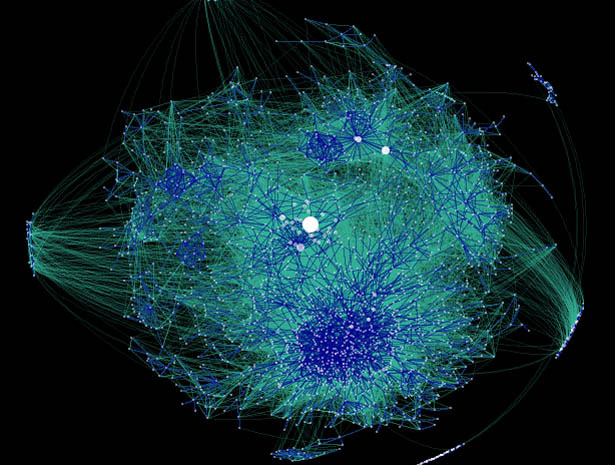
\includegraphics[width=11cm,height=6cm]{./figures/Internet3}
  	\caption{Affichage hyperbolique de blogs en utilisant à la fois les ensembles 
  	de données WWE et ICWSM 2007 (http://datamining.typepad.com/).}
  	\label{Internet}
  \end{figure}

  Il existe un certain nombre d'importantes raisons pratiques pour être intéressé à étudier la structure du réseau
  d'Internet. La fonction d'Internet consiste à transporter des données entre ordinateurs dans différentes parties du 
  monde, ce qui se fait en divisant les données en pièces ou en paquets et en les transportant d'un nœud à l'autre sur
  le réseau jusqu'à ce qu'ils atteignent leur destination, sans aucun doute, la structure du réseau affectera la manière
  dont il accomplit efficacement cette fonction et si nous connaissons la structure du réseau, nous pouvons aborder de
  nombreuses questions et problèmes de pertinence pratique.
  
\subsubsection{Réseaux Biologiques}
  Une autre classe des  réseaux les plus étudiées dans la littérature est celle des réseaux biologiques. Cette classe
  contient une grande variété de réseaux naturels. Le corps, qu'il soit humain ou animal, contient un grand nombre de 
  réseaux, dont certains se produisent dans l'espace réel, tels que le système nerveux. Ces réseaux ont été étudiés 
  depuis longtemps \cite{WB1997}. Une autre classe de réseau, ce sont les réseaux d'interactions gène-gène, 
  protéines-gène et protéines-protéines \cite{DM2003}, ainsi que les réseaux d'interactions entre les espèces dans
  les écosystèmes, comme la prédation ou la coopération.\\
\begin{figure}[h!]
\centering
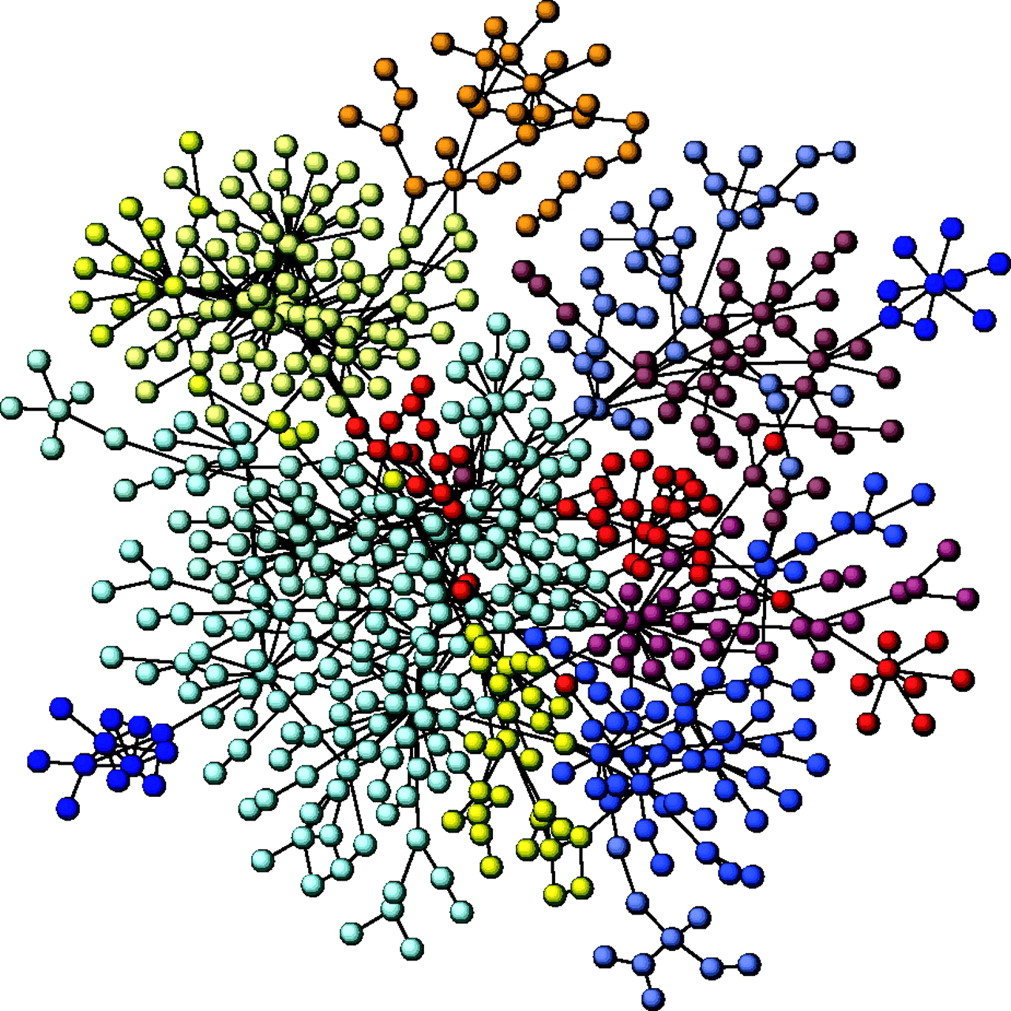
\includegraphics[scale=0.2]{./figures/PPI}
\caption{Un réseau modulaire est illustré au moyen du protéome humain (données obtenues à partir de la base
de données DIP: http://dip-doe-mbi.ucla.edu). Les nœuds sont des protéines et des liens indiquent leur 
interaction physique (protéine-protéine).}
\label{PPI}
\end{figure}
 La structure de ces réseaux se diffère selon chaque cas. Par exemple, les réseaux métaboliques sont des réseaux
 de protéines interagissant les uns avec les autres à l'intérieur de la cellule (Fig.~\ref{PPI}), il s'agit d'un réseau
 dirigé, car chaque protéine peut catalyser ou réprimer la création d'autres protéines, ce qui n'implique pas 
 nécessairement le processus inverse. La structure à grande échelle des réseaux métaboliques a été étudiée pour
 de nombreuses espèces, il a été trouvé que ces réseaux ont une distribution des degrés sans échelle \cite{Je-al2000}.
 De plus, il a été observé que le diamètre du réseau est très petit et presque indépendant de la taille du réseau, 
 cette indépendance s'explique par le fait que certain classe de réseaux sans échelle est Ultra-small
 \cite{Cohen-Havlin2003,Do-al2003,ChL2003}. Nos résultats du troisième chapitre renforcent 
 cette hypothèse et montrent que la dépendance du diamètre avec la taille du réseau peut devenir extrêmement faible.\\
 Dans les réseaux génétiques, les nœuds représentent des gènes, et les liens sont dirigés  et représentent
 l'influence d'un gène sur un autre, le réseau E. coli\footnote{Escherichia coli (en abrégé E. coli) sont des
 bactéries présentes dans l'environnement, les aliments et les intestins des humains et des animaux. E. coli est 
 un groupe important et diversifié de bactéries.} est un des réseaux génétiques qui est bien étudiés dans la 
 littérature \cite{Mi-al2002}.


 \subsubsection{Réseaux Sociaux}
  Un réseau social est un ensemble de nœuds, où ces nœuds se représente par des  personnes  (individus ou groupes sociaux)
  et les liens par une relation qui peut être de parenté, amitié, statut, etc \cite{JS2000}, cette diversité des liens
  est une chose appréciée dans l'étude des réseaux sociaux, car il existe de nombreuses définitions possibles d'un tel 
  réseau et la définition particulière que l'on utilisera dépendra des questions auxquelles on est intéressé à répondre.
  Tel que les réseaux d'amitiés entre les individus \cite{WW1977,Mo1934}, les relations d'affaires entre les entreprises
  \cite{JP1977}.
  La société offre une grande variété d'organisations de groupes possibles: les familles, les milieux de travail et
  d'amitié, les villages, les villes, les nations. La diffusion d'Internet a également conduit à la création de
  groupes virtuels, en direct sur le Web, comme Facebook qui relie des millons de personnes à travers le monde
  (voir Fig.~\ref{Facebook}).
  
\begin{figure}[h!]
\centering
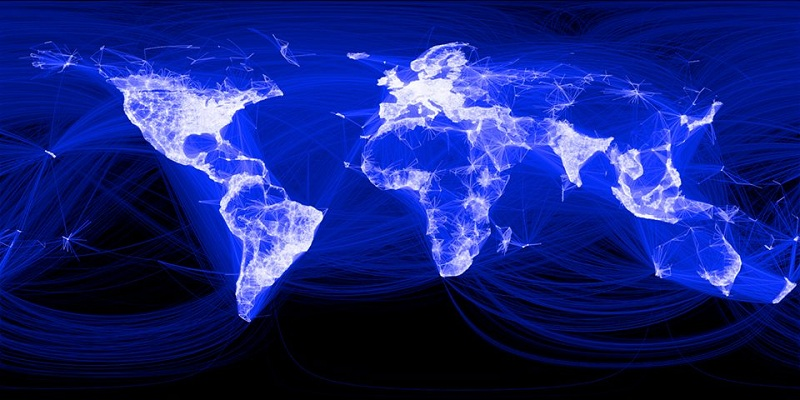
\includegraphics[width=9cm,height=5cm]{./figures/facebook}
\caption{Le graphe social derrière Facebook, graphe des relations d'amis de $500$ million de personnes, image par 
Paul Butley, $2010$.}
\label{Facebook}
\end{figure}
Bien avant que l'Internet commence à jouer un rôle important dans la vie de beaucoup de personnes, les sociologues
et d'autres chercheurs des sciences humaines ont examiné la structure des groupes de personnes. Dans la plupart des
cas, des groupes relativement petits ont été considérés, nécessairement parce que l'analyse de grands groupes n'était
pas souvent possible.\\
Une contribution importante à l'analyse des réseaux sociaux est venue de Jacob Moreno qui a introduit des sociogrammes
dans les années $1930$. Un sociogramme peut être considéré comme une représentation graphique d'un réseau: les personnes
sont représentées par des points (appelés nœuds) et leurs relations par des lignes reliant ces points (appelés liens).\\
L'analyse des réseaux sociaux a été importante pour le développement ultérieur de la théorie des graphes, par exemple 
en ce qui concerne l'introduction de mesures pour identifier l'importance des personnes ou des groupes. Par exemple,
une personne ayant de nombreuses connexions avec d'autres personnes peut être considérée comme relativement importante.
De même, une personne au centre d'un réseau semble être plus influente que quelqu'un au bord. Ce que la théorie des 
graphes nous fournit, ce sont les outils pour décrire formellement l'importance et l'influence des nœuds. En outre, 
en utilisant la théorie des graphes, nous pouvons facilement proposer des solutions alternatives pour décrire 
l'importance des personnes. L'existence de ces outils a également améliorer la précision des déclarations concernant
le poste ou le rôle de ces personnes au sein d'une communauté.
 \subsubsection{Réseaux d'informations}        
 Les  réseaux de citation et le World Wide Web (WWW), comme dans la Fig.~\ref{WWW}, sont un bon exemple des réseaux d'informations, car leur contenu d'informations étant stockée dans des nœuds, c’est pour cette raison que l’on utilise le terme réseau d’informations. Parfois on rencontre une certaine confusion à propos de réseau  WWW 
 et le réseau d'Internet. Dans la WWW, les nœuds sont les pages HTML, et les arêtes représentent les liens entre 
 les pages, par contre  dans l'Internet, les liens correspondent aux câbles physiques entre les ordinateurs. Alors le WWW est virtuelle et Internet est physique.
 
\begin{figure}[h!]
	\centering
	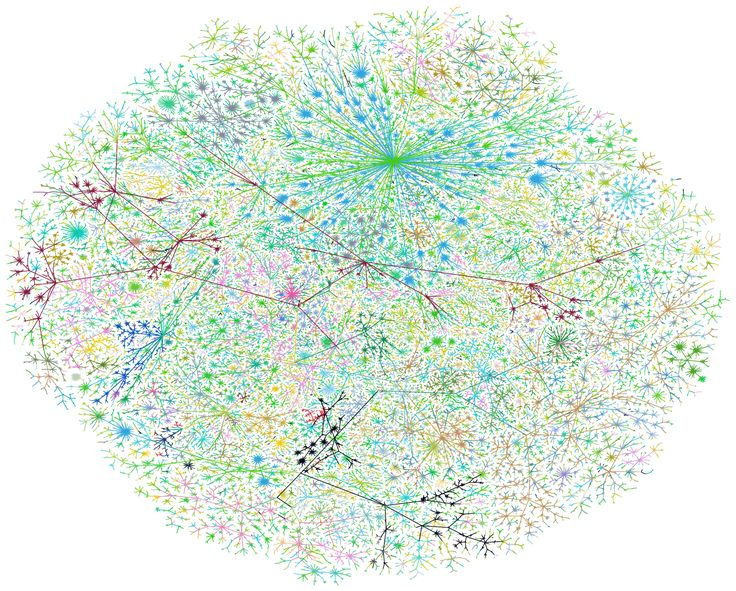
\includegraphics[scale=0.4]{./figures/www2}
	\caption{La structure de l'Internet au niveau des systèmes autonomes. Les nœuds de cette représentation sont des systèmes autonomes et les arêtes montrent les itinéraires empruntés par les données qui circulent entre eux. La photo a été créée par Hal Burch et Bill Cheswick en 2009.}
	\label{WWW}
\end{figure}

\section{Les réseaux complexes, la physique moderne et l'unification}
La physique explique les phénomènes de la nature en les réduisant à une interaction de lois fondamentales simples. Cette
méthode plutôt réussie semble rencontrer certaines difficultés lorsqu'il s'agit des systèmes complexes en général et des 
réseaux complexes en particulier. Dans ces derniers il reste peu clair s'il existe des lois universelles uniques expliquant
une variété de similitudes structurelles et dynamiques trouvées dans de nombreux réseaux réels différents  
\cite{K-al2012,BS2009,La-al2009,Li-al2011}. En revanche, l'\textsf{unification} des lois universelles qui paraissaient
jusqu'alors complètement séparées sont-elles d'une  origine commune ? c'est ce que les physiciens théoriques essaient de
découvrir. Une telle  \textsf{unification} va \^{e}tre, sans doute, un grand pas dans notre compréhension de la nature.
En outre, l'existence de cette idée au cœur de l'unification montre le pouvoir mystérieux que les êtres humains
peuvent découvrir derrière les apparences de la nature \cite{Sm1997}.\\
Le réseau causal représentant la structure à grande échelle de l'espace-temps dans notre univers accéléré est un graphe de 
loi de puissance avec un regroupement fort, similaire à de nombreux réseaux complexes tels que les réseaux Internet, 
sociaux ou biologiques \cite{K-al2012}. Cette similitude structurelle est une conséquence de l'équivalence asymptotique
entre la dynamique de croissance à grande échelle des réseaux complexes et des réseaux causaux. Par conséquent, un intérêt 
croissant est adressé à l'étude de la gravité quantique à partir de la théorie de l'information et de la perspective des 
réseaux complexes \cite{Tr2015,Bi-al2015}. Récemment, des relations intrigantes entre les propriétés des réseaux de 
communication quantique avec des topologies du réseau et la physique statistique ont été rapportées. Sur la base des
concepts classiques de percolation \cite{BR2006}, il a été montré que ces réseaux quantiques peuvent présenter une
transition de phase de percolation d'enchevêtrement \cite{Ac-al2007,Sa1999}.
L'avancement rapide de la technologie de l'information quantique a suscité un intérêt considérable pour les propriétés 
dynamiques des réseaux quantiques formés par les systèmes élémentaires, tels que les qubits, en raison de leur rôle
privilégié dans la communication et le calcul quantiques \cite{J-al2015,BG2007,MC2000}.\\

%Un autre domaine de recherche en relation avec les sciences des réseaux et notamment aux réseaux complexes. 
La science générale des réseaux et de ses diverses applications a une pertinence significative pour les praticiens de 
l'intelligence artificiel (IA). Par exemple, la compréhension de la structure d'Internet et du World Wide Web est importante 
pour l'orientation de la direction de l'intelligent, l'équilibrage de charge, la recherche de toutes sortes et le 
déploiement d'agents\footnote{Un agent est un terme important en IA qui désigne une entité capable d’interagir avec
son environnement.} intelligents qui assistent les utilisateurs dans leurs tâches réseau. La réflexion en
réseau sera également fondamentale pour développer des algorithmes décentralisés efficaces pour les réseaux de calcul,
de communication et de détection de plus en plus distribués et liés, ainsi que des méthodes de sécurité efficaces pour 
ces systèmes de plus en plus vulnérables. Ce sont tous des domaines dans lesquels la recherche sur l'IA et 
l'apprentissage automatique ont joué et joueront un rôle majeur \cite{Mitchell2006,Basheer-Hajmeerb2000,Passerini-al2017}.

\section{La théorie des graphes}
En terme générale, un réseau se décrit comme un graphe dont les nœuds (sommets) identifient les éléments du
système et les liens de connexion (arêtes) représente la présence d'une relation ou d'une interaction entre ces
éléments. Avec un tel niveau de généralité, il est facile de percevoir qu'un large éventail de systèmes peuvent 
être abordés dans le cadre de la théorie du graphe. Alors nous fournissons ici un bref historique et quelques 
notations de base nécessaires dans la théorie de graphe pour décrire les réseaux. Le cadre naturel pour une description
mathématique rigoureuse des réseaux se trouve dans la théorie des graphes, mais il faut noter que la théorie des graphes 
constitue une branche des mathématiques importante et nous n'allons pas fournir une présentation
formelle et complète de  celle-ci (voir \cite{Ha1995,West1996} par exemple). Cependant notre but dans ce chapitre 
d'introduction est de fournir seulement quelques notions utiles pour décrire les réseaux dans la suite de cette thèse.
  \subsection{Bref historique}
  En plus de la topologie, Euler est devenue le père de la théorie des graphes quand il a résolu, en $1736$, un problème 
  célèbre sous le nom \textit{"le problème du pont de K\"{o}nigsberg"}, la question était de savoir s'il était possible 
  de visiter les quatre quartiers de la ville séparés les uns des autres par un bras de rivière, en passant exactement
  une fois par chaque pont et en revenant à son point de départ (voir Fig.~\ref{Konig}).
  
\begin{figure}[h!]
\centering
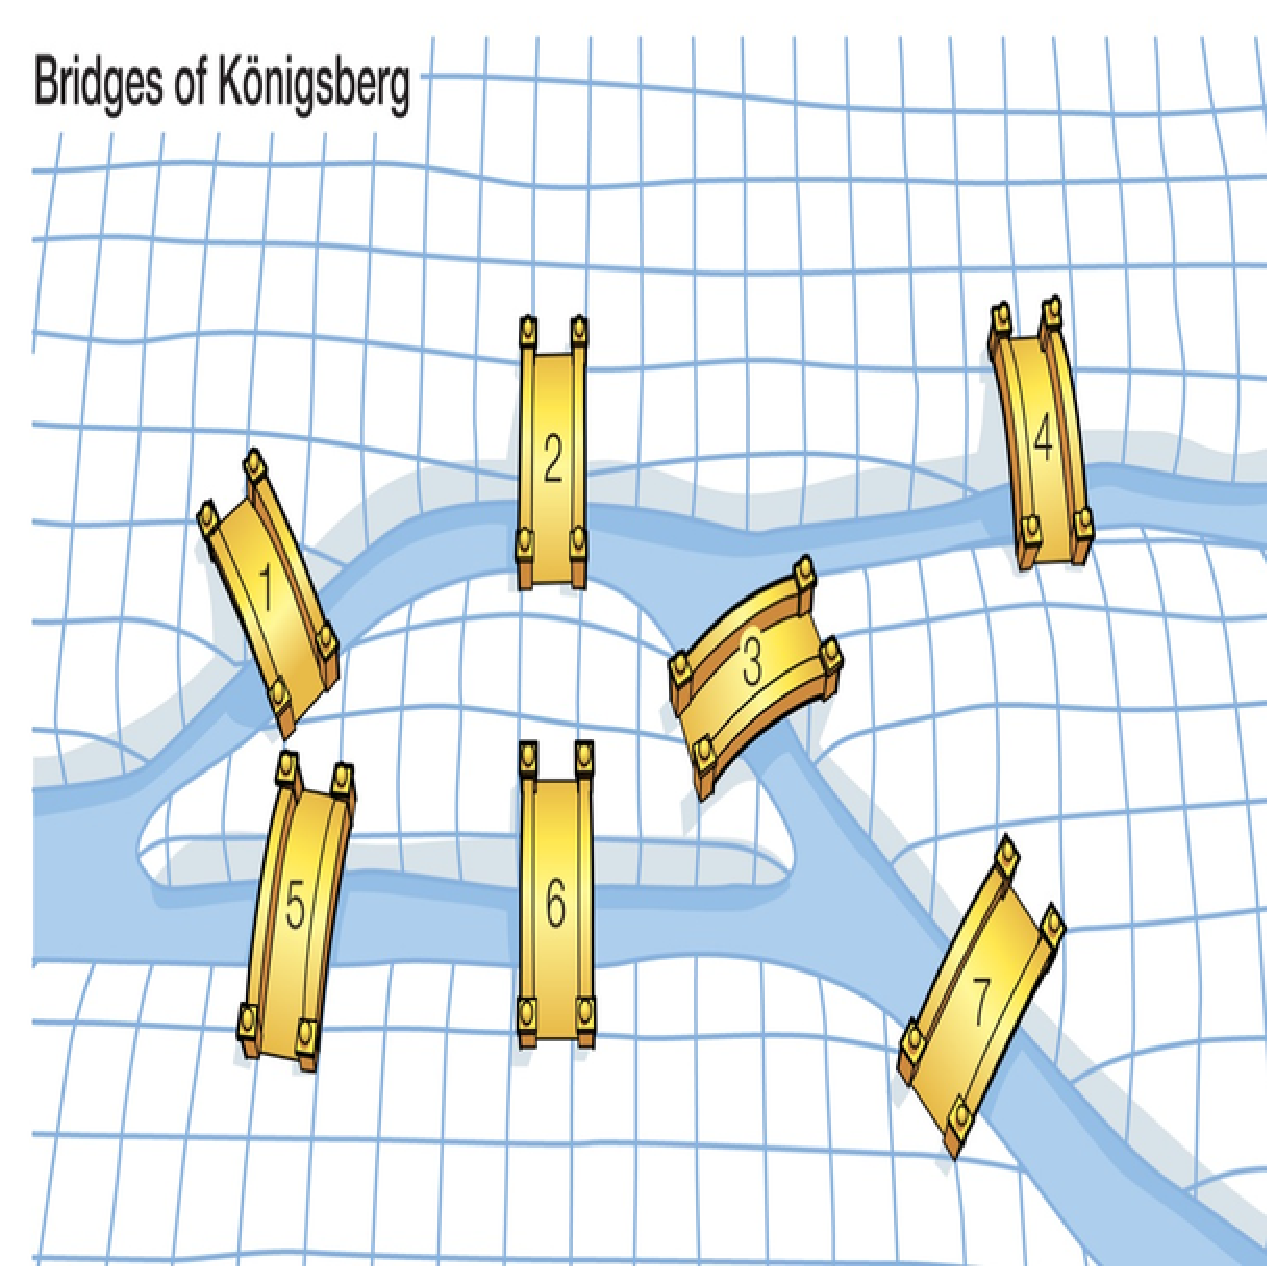
\includegraphics[scale=0.7]{./figures/Konig}
\caption{Ponts de K$\ddot{o}$nigsberg, $1736$}
\label{Konig}
\end{figure}
Afin de trouver une solution à ce problème Euler a remplacé chaque zone de terrain par un point et chaque pont par une 
ligne  joignant les points correspondants, produisant ainsi un \textit{"graphe"}. Ainsi il a montré que le problème
est insoluble et que le graphe de cette ville ne peut pas être parcouru d'une certaine manière.

En $1847$ Kirchhoff a développé la théorie des arbres afin de résoudre le système d'équations linéaires simultanées qui 
donnent le courant dans chaque branche et autour de chaque circuit d'un réseau électrique. Bien qu'un physicien, il a 
pensé comme un mathématicien lorsqu'il a remplacé un réseau électrique par sa structure combinatoire  correspondante 
constituée uniquement de points et de lignes sans indication du type d'élément électrique représenté par des lignes
individuelles. Dans les années $1960$, deux mathématiciens, Paul Erd\H{o}s et Alfred Rényi (ER), ont introduit une 
nouvelle idée ingénieuse, ils ont combiné les concepts de la théorie des graphes avec les outils de la théorie des 
probabilités, ce qui permet d'envisager des familles de graphes plutôt que des graphes spécifiques.

 \subsection{L’expérience de Milgram}
 \label{Milgram} 
En $1967$, Stanley Milgram a effectué une expérience intéressante.  Dans sa première expérience, Milgram a demandé à des
personnes choisies au hasard au Nebraska d'envoyer des lettres à une personne cible éloignée à Boston.
Les participants ne pouvaient passer que les lettres (à la main) aux connaissances personnelles qu'ils pensaient pouvoir 
atteindre la cible, soit directement, soit via un  "ami d'un ami".  Dans sa première experience seules trois lettres ont
finalement atteint leur destination. Mais dans les expériences ultérieures, Milgram a réussi à augmenter
le taux de réussite à $95\%$, pour plus de détails (voir \cite{Mi1967,TM1969}). La conclusion principale du cette
expérience de Milgram était que la plupart des gens sur notre planète n'est séparé que par six autres personnes en moyenne.
Cette idée de Milgram a été reprise encore une fois en 2001 par Duncan Watts et ses collègues en utilisant un message 
électronique qui devait être livré à des expéditeurs autour de monde, étonnamment, Watts a constaté que le nombre moyen 
d'intermédiaires était $6$. Pour plus de détails et une analyse statistique beaucoup plus étendue des données par rapport
à l'analyse de Milgram, voir Dodds et al \cite{D-al2003}.

\subsection{Représentation d'un graphe}
  Un graphe est un ensemble de points nommés nœuds ou sommets  reliés par des traits 
  nommées arêtes (ou liens ou arcs). L'ensemble des arêtes entre nœuds forme une figure similaire à un 
  réseau. Un  graphe $G(V,E)$ est alors défini par un couple $(V,E)$, où $V$ (vertices en anglais) désigne
  l'ensemble des nœuds et $E$ (edges en anglais) l'ensemble des liens.
 
  \subsubsection{La matrice d’adjacence}
 Un graphe est représenté fréquemment par une matrice d'adjacence, $M_{i,j}$, dans laquelle chaque ligne et
 chaque colonne représente un nœud du graphe. Dans un graphe non-orienté l'élément $M_{i,j}=1$ si un lien existe
 entre le $i^{eme}$ et le $j^{eme}$ nœud sinon $M_{i,j}=0$  (voir Fig.~\ref{matrice d'adjacence}), ainsi la matrice 
 sera en général symétrique et les éléments diagonaux sont nécessairement $0$.
  \begin{figure}[h]
 	\centering
 	\subfloat{
 		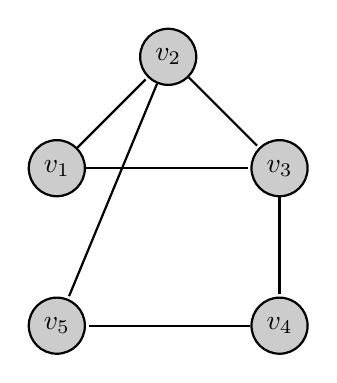
\begin{tikzpicture}[shorten >=1pt,auto,node distance=2cm,thick,main node/.style={circle,fill=black!20,draw}]
 		%[-,>=stealth',shorten >=1pt,auto,node distance=2cm,thick,main node/.style={circle,fill=black!20,draw}]
 		\node[main node] (1) {$v_2$};
 		\node[main node] (2) [below left of=1] {$v_1$};
 		\node[main node] (3) [below right of=1] {$v_3$};
 		\node[main node] (4) [below of=3] {$v_4$};
 		\node[main node] (5) [below of=2] {$v_5$};
 		
 		\path[every node/.style={font=\sffamily\small}]
 		(2) edge node [left] {} (1)
 		(2) edge node [left] {} (3)
 		(1) edge node [left] {} (5)
 		(1) edge node [left] {} (3)
 		(3) edge node [left] {} (4)
 		(4) edge node [left] {} (5)
 		;
 		\end{tikzpicture}}
 	\subfloat{
 		\vbox{\hbox{
 				\begin{math}
 				M_{G} = \left(
 				\begin{array}{ccccc}
 				0 & 1 & 1 & 0 & 0 \\
 				1 & 0 & 1 & 0 & 1 \\
 				1 & 1 & 0 & 1 & 0 \\
 				0 & 0 & 1 & 0 & 1 \\
 				0 & 1 & 0 & 1 & 0
 				\end{array}
 				\right)
 				\end{math}
 			}% end of first hbox
 			\null% last null hbox, which sets the baseline of the \vbox
 		} % end of vbox
 	} % end of subfloat
 	\caption{Exemple d'un graphe non-orienté et sa matrice d'adjacence $M_G$ avec 5 nœuds et 6 liens.}
 	\label{matrice d'adjacence}
 \end{figure}  
 
  Un graphe orienté est un graphe où les arêtes  sont dirigés, c'est-à-dire que chaque bord est une paire de nœuds ordonnée avec ($i$,$j$) désignant un bord (flèche) qui commence au nœud $i$ et se termine au nœud $j$ 
  (Fig.~\ref{matrice d'adjacence2}). 
 
 \begin{figure}[h]
	\centering
	\subfloat{
		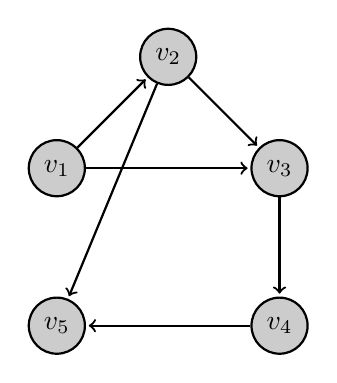
\begin{tikzpicture}[->,shorten >=1pt,auto,node distance=2cm,thick,main node/.style={circle,fill=black!20,draw}]
		%[-,>=stealth',shorten >=1pt,auto,node distance=2cm,thick,main node/.style={circle,fill=black!20,draw}]
		\node[main node] (1) {$v_2$};
		\node[main node] (2) [below left of=1] {$v_1$};
		\node[main node] (3) [below right of=1] {$v_3$};
		\node[main node] (4) [below of=3] {$v_4$};
		\node[main node] (5) [below of=2] {$v_5$};
		
		\path[every node/.style={font=\sffamily\small}]
		(2) edge node [left] {} (1)
		(2) edge node [left] {} (3)
		(1) edge node [left] {} (5)
		(1) edge node [left] {} (3)
		(3) edge node [left] {} (4)
		(4) edge node [left] {} (5)
		;
		\end{tikzpicture}}
	\subfloat{
		\vbox{\hbox{
				\begin{math}
				M_{G} = \left(
				\begin{array}{ccccc}
				0 & 0 & 0 & 0 & 0 \\
				1 & 0 & 0 & 0 & 0 \\
				1 & 1 & 0 & 0 & 0 \\
				0 & 0 & 1 & 0 & 0 \\
				0 & 1 & 0 & 1 & 0
				\end{array}
				\right)
				\end{math}
			}% end of first hbox
			\null% last null hbox, which sets the baseline of the \vbox
		} % end of vbox
	} % end of subfloat
	\caption{Exemple d'un graphe orienté et sa matrice d'adjacence $M_G$ avec 5 nœuds et 6 liens.}
	\label{matrice d'adjacence2}
\end{figure}


\subsubsection{La liste d’adjacence}
Une représentation par liste d'adjacence d'un graphe associe, à chaque sommet du graphe, la collection de 
ses voisins, comme sommets ou comme arêtes.\\
\begin{figure}[h]
	\centering
	\subfloat{
		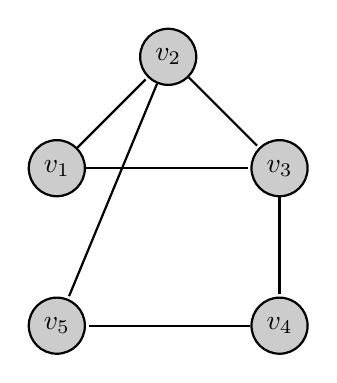
\begin{tikzpicture}[shorten >=1pt,auto,node distance=2cm,thick,main node/.style={circle,fill=black!20,draw}]
		%[-,>=stealth',shorten >=1pt,auto,node distance=2cm,thick,main node/.style={circle,fill=black!20,draw}]
		\node[main node] (1) {$v_2$};
		\node[main node] (2) [below left of=1] {$v_1$};
		\node[main node] (3) [below right of=1] {$v_3$};
		\node[main node] (4) [below of=3] {$v_4$};
		\node[main node] (5) [below of=2] {$v_5$};
		
		\path[every node/.style={font=\sffamily\small}]
		(2) edge node [left] {} (1)
		(2) edge node [left] {} (3)
		(1) edge node [left] {} (5)
		(1) edge node [left] {} (3)
		(3) edge node [left] {} (4)
		(4) edge node [left] {} (5)
		;
		\end{tikzpicture}}
	\subfloat{
		\vbox{\hbox{
				\begin{math}
				\begin{tabular*}{0.5\textwidth}{@{\extracolsep{\fill}}ccc} \toprule Noueds & voisins\\ \midrule 1	& 2,3\\ 2	& 1,3,5\\ 3	& 1,2,4\\ 4	& 3,5\\ 5 & 2,4 \\ \bottomrule
				\end{tabular*}			
				\end{math}
			}% end of first hbox
			\null% last null hbox, which sets the baseline of the \vbox
		} % end of vbox
	} % end of subfloat
	\caption{Exemple d'un graphe non-orienté et sa liste d'adjacence avec 5 nœuds et 6 liens.}
	\label{matrice d'adjacence1}
\end{figure}

En règle générale, les matrices sont utilisées pour les tableaux denses et les listes d'adjacence pour les 
tableaux dispersés. La raison est que les matrices consomment moins d'espace pour les tableaux denses et les listes
d'adjacence consomment moins d'espace pour les tableaux dispersés. Cependant, l'espace n'est qu'une considération, d'autres
facteurs doivent également être pris en compte.


\section{Caractéristiques des réseaux complexes}
Chaque réseau complexe présente des caractéristiques topologiques spécifiques qui caractérisent sa
connectivité et influencent fortement la dynamique des processus exécutés sur le réseau. L'analyse  et 
la synthèse des réseaux complexes reposent donc sur l'utilisation de mesures capables d'exprimer les caractéristiques
topologiques les plus pertinentes. La description quantitative des propriétés des réseaux fournit des
outils fondamentaux pour la classification des réseaux théoriques et réels en grandes catégories. Dans ce paragraphe 
nous introduisons quelques grandeurs ``microscopiques'' pour quantifer et analyser les réseaux complexes.

   \subsection{Plus court chemin}
   
   Le plus court chemin entre deux nœuds d'un graphe est défini comme étant la longueur du trajet le plus court parmi tous les trajets possibles. Une
   mesure statistique globale de la distance entre les nœuds peut alors être exprimée comme la valeur moyenne des chemins les
   plus courts entre tous les couples possibles de nœuds du réseau, mathématiquement on peut le définir par la forme suivante
   \begin{equation}
    \textless l\textgreater=\frac{1}{n(n-1)}\sum_{i,j} d_{i,j},
   \end{equation}
   avec $d_{ij}$ est la distance la plus courte du nœud $i$ au nœud $j$ et $n$ est le nombre total de nœuds dans le réseau. Sachant que la distance entre deux nœuds qui ne sont pas atteignables de l'un à l'autre est $0$  et la distance d'un nœud à lui-même est également $0$.\\
   Dans de nombreux réseaux à grande échelle, la distance moyenne entre les nœuds est très faible par rapport à la taille du graphe, ce phénomène est connu sous le nom de la propriété \textit{petit-monde}. Cette propriété a été popularisée dans le contexte sociologique où elle est parfois appelée \textit{six degrés de séparation}\cite{Mi1967}.\\
   L'importance de cette propriété consiste en son rôle important dans le transport et la communication au sein d'un réseau. Supposons qu'il soit nécessaire d'envoyer un paquet de données d'un ordinateur à un autre via Internet: la géodésique fournit un chemin  optimal, car on pourrait obtenir un transfert rapide et conserver les ressources du système \cite{PV2004}. Pour une telle raison, les chemins les plus courts ont également joué un rôle important dans la caractérisation de la structure interne d'un graphe \cite{Wa1994,JS2000,Bo-al2006}.

   Les ensembles de données massifs du réseau s'accumulent à un rythme énorme dans des champs variés \cite{Qi-al2010}. En utilisant la mesure moyenne du plus court chemin, les réseaux de petit-monde peuvent être considérés comme des systèmes à la fois efficaces à l'échelle mondiale et locale \cite{Latora-Marchiori2001}. Nous utilisons souvent la longueur du plus court chemin comme mesure de l'efficacité du réseau, ce qui nous permet de donner une analyse quantitative précise de l'efficacité du flux d'information dans les réseaux. Le calcul du plus court chemin a également été utilisé pour estimer la précision des approximations analytiques de la dynamique sur les réseaux \cite{Melnik-al2011}, en examinant l'apparition de la synchronisation \cite{Zhao-al2006} et en évaluant la résilience des réseaux de communication aux attaques et aux échecs \cite{Albert-al2000}.
   
   \subsection{Coefficient de regroupement (Clustering)}
   En plus de l'effet du petit-monde un haut niveau de regroupement s'en accompagne dans de nombreux
   réseaux sociaux et différents autres réseaux ont montré cette tendance également, notamment le réseau Internet \cite{Lad1999}, les réseaux de transport \cite{Seb-al2022} et les réseaux métaboliques \cite{WD2000,SC2001}.
   Le concept de regroupement d'un graphe
   se réfère à la tendance observée dans de nombreux réseaux naturels à former des cliques au voisinage d'un nœud donné, 
   cette propriété est appelée également la transitivité dans le contexte de la sociologie \cite{Wa1994}.\\
   Le coefficient de regroupement peut être considéré comme la fraction de paires de nœuds avec un nœud commun
   ou équivalent comme la probabilité moyenne que deux nœuds voisins ont un nœud commun, c'est peut-\^{e}tre la manière
   la plus utile de définir le coefficient de regroupement. En notation mathématique:
    \begin{equation}
    C=\frac{3\times\text{(Nombre de triangles)}}{\text{(Nombre de triplets connectés)}}
    \label{Clustering}.
   \end{equation}
   Le facteur $3$ dans le numérateur compense le fait que chaque triangle complet de trois nœuds contribue à trois triplets
   connectés, l'un centré sur chacun des trois nœuds et assure que $0\leq C\leq 1$.
 
 
 \begin{figure}[h!]
   \begin{center}
   \begin{tikzpicture}
   \tikzset{main node/.style={circle,fill=blue!20,draw,minimum size=0.5cm,inner sep=0pt},
            }
    \begin{scope}[xshift=1.5cm]
    \node[main node] (1) {};
    \node[main node] (2) [right = 1cm  of 1]  {};
    \node[main node] (3) [below = 1cm  of 1] {};
    \node[main node] (4) [right = 1cm  of 3] {};

    \path[draw,thick]
    (1) edge node {} (2)
    (4) edge node {} (3)
    (3) edge node {} (1)
    (4) edge node {} (2);
     \end{scope}
    \begin{scope}[xshift=5cm]
    \node[main node] (1) {};
    \node[main node] (2) [right = 1cm  of 1]  {};
    \node[main node] (3) [below = 1cm  of 1] {};
    \node[main node] (4) [right = 1cm  of 3] {};

    \path[draw,thick]
    (1) edge node {} (2)
    (1) edge node {} (3)
    (3) edge node {} (2)
    (3) edge node {} (4)
    ;
    \end{scope}
    \begin{scope}[xshift=8.5cm]
     \node[main node] (1) {};
    \node[main node] (2) [right = 1cm  of 1]  {};
    \node[main node] (3) [below = 1cm  of 1] {};
    \node[main node] (4) [right = 1cm  of 3] {};
    
    \path[draw,thick]
    (1) edge node {} (2)
    (1) edge node {} (3)
    (1) edge node {} (4)
    (2) edge node {} (3)
    (2) edge node {} (4)
    (3) edge node {} (4)
    ;
    \end{scope}
\node[text width=2cm] at (2.7,-2.2) {$C=0$};
\node[text width=2cm] at (6.1,-2.2) {$C=7/12$};
\node[text width=2cm] at (9.7,-2.2) {$C=1$};
\end{tikzpicture}
\end{center}
   \caption{ Exemple de coefficient de regroupement.}
\label{Clustering}
\end{figure}

Une autre définition du coefficient de regroupement, également largement utilisé, a été donnée par Watts et Strogatz \cite{WS1998},
qui a proposé de définir une valeur locale
 \begin{equation}
    C_i=\frac{\text{(Nombre de triangles connectés au nœud $i$)}}{\text{(Nombre de triples centrés sur le nœud $i$)}}.
  \end{equation}
  Dans le cas où le nœud a le degré $0$ ou $1$, nous mettons $C_i=0$, Ensuite, le coefficient de regroupement pour l'ensemble
  du réseau est la moyenne
  \begin{equation}
    C=\frac{1}{n}\sum_i C_i.
  \end{equation}
 Le coefficient de regroupement mesure la densité des triangles dans un réseau. Une généralisation évidente a été envisagée à 
propos de la densité des boucles plus longues que trois, boucles de longueur quatre et plus. Un certain nombre d'auteurs ont 
examiné ces coefficients de regroupement d'ordre supérieur \cite{Ne2003,BC2003,Fron-al2002,Gle-al2001}, bien qu'il n'y ait jusqu'à présent
aucune théorie propre qui sépare les contributions indépendantes des différents ordres l'un de l'autre.
 %\vspace{2 cm}
   \subsection{Distribution des degrés}
   La propriété la plus importante qui caractérise une structure de réseau est la distribution des degrés $P(k)$,
   définie comme la probabilité qu'un nœud choisi uniformément au hasard ait un degré $k$ ou, de manière équivalente, la
   fraction de nœuds dans le graphe ait le degré $k$.
   Si le graphe est dirigé, le degré du nœud comporte deux composantes: le nombre de liens sortants $k^{out}$ (appelé
   "out-degree") et le nombre de liens entrants $k^{in}$ (appelé "in-degree"). Le degré total est alors défini comme 
   $k=k^{out}+k^{in}$.\\
%   \begin{figure}[h!]
%   	\centering
%   	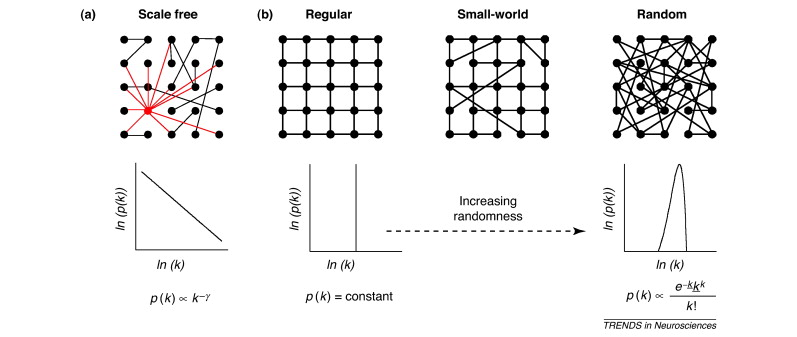
\includegraphics[width=12cm,height=8cm]{./figures/distribution-degree}
%   	\caption{.}
%   	\label{distribution-degree}
%   \end{figure}

Un réseau ordinaire a une séquence de degré simple parce que tous les nœuds ont le même nombre de arêtes, et donc une forme de distribution des degrés qui contient une seule pointe forte. En outre dans le cas d'un réseau complètement aléatoire, 
la séquence de degré obéit à la distribution de Poisson qui diminue exponentiellement, loin de la valeur moyenne $\textless k\textgreater$. En raison de ce déclin exponentiel, la probabilité de trouver un nœud avec $k$ bord devient négligeable pour  $k\gg \textless k\textgreater$.
Au cours des dernières années, de nombreux résultats empiriques ont montré que pour la plupart des réseaux réels à grande échelle, la distribution des degrés s'écarte de manière significative de la distribution de Poisson.\\
En particulier, pour un certain nombre de réseaux, la distribution des degrés peut être mieux décrite par une loi de puissance de la forme $P(k)\sim k^{-\gamma}$. Cette distribution de la loi de puissance diminue progressivement et permet de créer quelques nœuds de très grande importance. Étant donné que ces lois de puissance sont libres de toute échelle caractéristique, un tel réseau est appelé un réseau sans échelle.

\subsection{Degré de corrélation} 
Un grand nombre de réseaux réels sont corrélés dans le sens que la probabilité qu'un nœud de degré $k$ soit connecté à un autre
nœud de degré, disons $k'$, dépend de $k$. Dans ces cas, il est nécessaire d'introduire la probabilité conditionnelle 
$P(k'\backslash k)$, étant défini comme la probabilité qu'un lien d'un nœud de degré $k$ soit connecté à un nœud de degré 
$k'$ \cite{BP2002}. Bien que les corrélations de degré soient formellement caractérisées par $P(k'\backslash k)$, l'évaluation directe de la probabilité conditionnelle donne des résultats extrêmement bruyants pour la plupart des réseaux réels en raison de leur taille finie $n$. Ce problème peut être surmonté en définissant le degré moyen des voisins les plus proches d'un nœud $i$
comme
\begin{equation}
 k_{nn,i}=\frac{1}{k_i}\sum_{j\in n_i}k_j,
\end{equation}
où la somme s'exécute sur les nœuds appartenant à $n_i$ qui signifie l'ensemble des premiers voisins de $i$. on peut calculer le degré 
moyen des voisins les plus proches des nœuds avec le degré $k$, noté $k_{nn}(k)$, obtenant une expression qui intègre implicitement
la dépendance de $k$. Une telle quantité peut, en effet, être exprimée en termes de probabilité conditionnelle comme
\begin{equation}
 k_{nn}(k)=\sum_{k'}k'P(k'\backslash k).
 \label{knn}
\end{equation}
S'il n'y a pas de corrélation de degré, l'Eq.~\eqref{knn} donne
$k_{nn}(k)=\frac{\textless k^2\textgreater}{\textless k\textgreater}$, c'est-à-dire que $k_{nn}(k)$ est indépendant de $k$
\cite{Bo-al2006}.\\
\begin{figure}[h!]
	\centering
	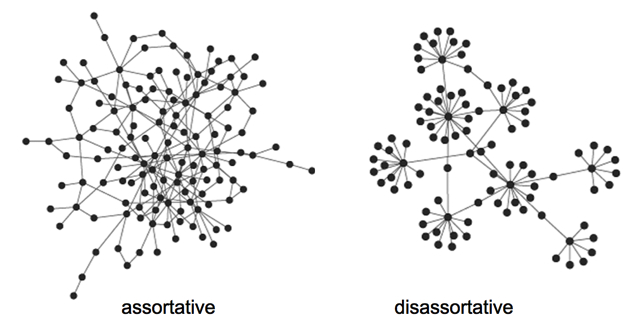
\includegraphics[scale=0.6]{./figures/assortative_disassortative}
	\caption{Exemple des réseaux assortatif et disassortatif.}
	\label{assortative_disassortative}
\end{figure}
\label{s-correl}

Selon l'Eq.~\eqref{knn} on peut distinguer deux différents types de réseaux, si les nœuds de haut degré dans un réseau  s'associent préférentiellement avec d'autres nœuds à haut degré on dit que le réseau est assortatif, et s'ils préfèrent  s'attacher à ceux à faible degré on dit que le réseau est disassortatif (voir Fig.~\ref{assortative_disassortative}). Les deux situations sont observées dans certains réseaux, mais le cas du réseau assortatif est particulièrement intéressant, car le degré est lui-même une propriété de la topologie des graphes, alors les corrélations de degré peuvent donner lieu à des effets de structure du réseau intéressants \cite{MS2002,Ne2003}. 

\subsection{Mesures de la centralité}

L'identification des nœuds importants dans les réseaux est un problème intéressant qui a suscité beaucoup d'attention, surtout dans le contexte des réseaux de communication. Par exemple, la communication entre un groupe d'humains forme un réseau de communication \cite{Dehmer2011}. Les sciences sociales à la fin des années 1940 ont développé des mesures théoriques pour détecter des nœuds importants dans les réseaux. Une classe importante de ces mesures est basée sur le concept de centralité \cite{Hage-Harary1995,Wasserman-Faust1994} qui tente intuitivement d'identifier les nœuds qui sont au centre de la communication au sein du réseau parmi tous les nœuds. Il existe deux types fondamentalement différents de mesures de centralité \cite{Freeman1977}. Le premier type évalue la centralité de chaque nœud dans un réseau et s'appelle des mesures de centralité des points où le mot "point" se réfère à un nœud ou un sommet. Le second type s'appelle les mesures de centralité des graphes car il attribue une valeur de centralité à l'ensemble du réseau. Parmi les paramètre du mesure de centralité on cite:\\

%\subsubsection{Centralité d'intermédiarité (Betweenness)}
\begin{itemize}
 \item[i)] Centralité d'intermédiarité (Betweenness):\\
  L'importance d'un nœud dans un réseau dépend de nombreux facteurs. Un site Web peut être important en raison de son contenu, d'un routeur pour sa capacité, d'un métabolite dû à sa fonction biochimique, etc. Bien sûr, toutes ces propriétés dépendent de la nature du réseau étudié et peuvent avoir très peu à faire avec la structure graphique du réseau. L'une des définitions les plus acceptées de centralité est basée sur les chemins de comptage traversant un nœud $i$ dans le réseau, on compte le nombre de chemins de "routage" vers tous les autres nœuds passant par $i$, et ce nombre détermine la centralité $i$. La sélection la plus courante ne prend que les chemins les plus courts en tant que chemins de routage. Cela conduit à la définition suivante: la centralité de l'intermédiarité d'un nœud $i$ équivaut au nombre de chemins les plus courts entre toutes les paires de nœuds dans le réseau qui l'entoure, c'est-à-dire,
 \begin{equation}
 C_B(i)=\sum_{l\neq j}\dfrac{\sigma_{lj}(i)}{\sigma_{lj}},
 \end{equation}
 
 avec $\sigma_{lj}$ indique le nombre des plus court chemins de $l$ à $j$, et $\sigma_{lj}(i)$ indique le nombre des plus court chemins de $l$ à $j$ passant par $i$.
 
%\subsubsection{La centralité de proximité}
\item[ii)] La centralité de proximité:\\
La centralité de proximité tente de mesurer la proximité d'un nœud avec d'autres nœuds du réseau. Ceci se fait en termes de distance de communication mesurée par le nombre d'arêtes entre deux nœuds si connecté par le chemin le plus court.
\begin{equation}
C_C(i)=\dfrac{1}{\sum_{j=1}^nd_{ji}},
\end{equation}
$d_{ji}$ est le plus court chemin entre le nœud $j$ et $i$.

En ce qui concerne la centralité de proximité, les gens se réfèrent généralement à sa forme normalisée qui représente la longueur moyenne des chemins les plus courts au lieu de leur somme. Il est généralement donné par la formule précédente multipliée par $n-1$. Pour les larges réseaux de très grand nombre de nœuds on écrit:
\begin{equation}
C_C(i)=\dfrac{n}{\sum_{j=1}^nd_{ji}}.
\end{equation}
\end{itemize}

\section{Propriétés des réseaux réels}
\subsection{La propriété petit-monde}
La propriété petit monde se réfère au fait que dans plusieurs réseaux, peut-être la plupart des réseaux à grande échelle, la distance moyenne entre les nœuds est très faible par rapport à la taille des graphes. La distance entre deux nœuds d'un graphe est mesurée comme la plus petite longueur de chemin entre eux. Une mesure statistique globale de la distance entre les nœuds peut alors être exprimée comme la longueur moyenne des trajets  les plus courts pour tous les couples possibles de nœuds dans le réseau. Nous avons mentionné dans la Section.~\ref{Milgram} l'expérience de Stanley Milgram réalisée dans les années $1960$, dans laquelle on a trouvé que le nombre d'étapes pour qu'un destinataire reçoive la lettre de l'expéditeur, via le réseau social, est égale à six en moyenne. L'expérience de Milgram est une démonstration simple, magnifique et puissante de l'effet de petit-monde.\\
L'effet petit-monde a des implications évidentes pour la dynamique des processus qui se déroulent sur les réseaux. Par exemple, si l'on considère la diffusion de l'information, ou encore tout autre chose, à travers un réseau, l'effet petit-monde implique que cette propagation sera rapide sur la plupart des réseaux réels. Cela affecte le nombre de "sauts" qu'un paquet doit faire pour passer d'un ordinateur à l'autre sur Internet, le nombre d'escales d'un voyage pour un voyageur aérien ou en train, le temps qu'il faut pour qu'une maladie se propage dans
une population, et ainsi de suite. L'effet petit-monde atteint également certains jeux de société bien connus, en particulier le calcul des nombres d'Erd\H{o}s \cite{RG1999} et de Bacon.

\subsection{La distribution des degrés sans échelle}
\label{s-libre-echelle}
La distribution des degrés sans échelle qu'on appelle également la loi de puissance a suscité un intérêt particulier au cours des dernières années pour ses propriétés mathématiques, ce qui entraîne parfois des conséquences physiques surprenantes et son apparence dans la diversité des réseaux naturels et artificiels, voir quelques exemples dans la Fig.~\ref{scal-free-reels}.\\

\begin{figure}[h!]
\centering
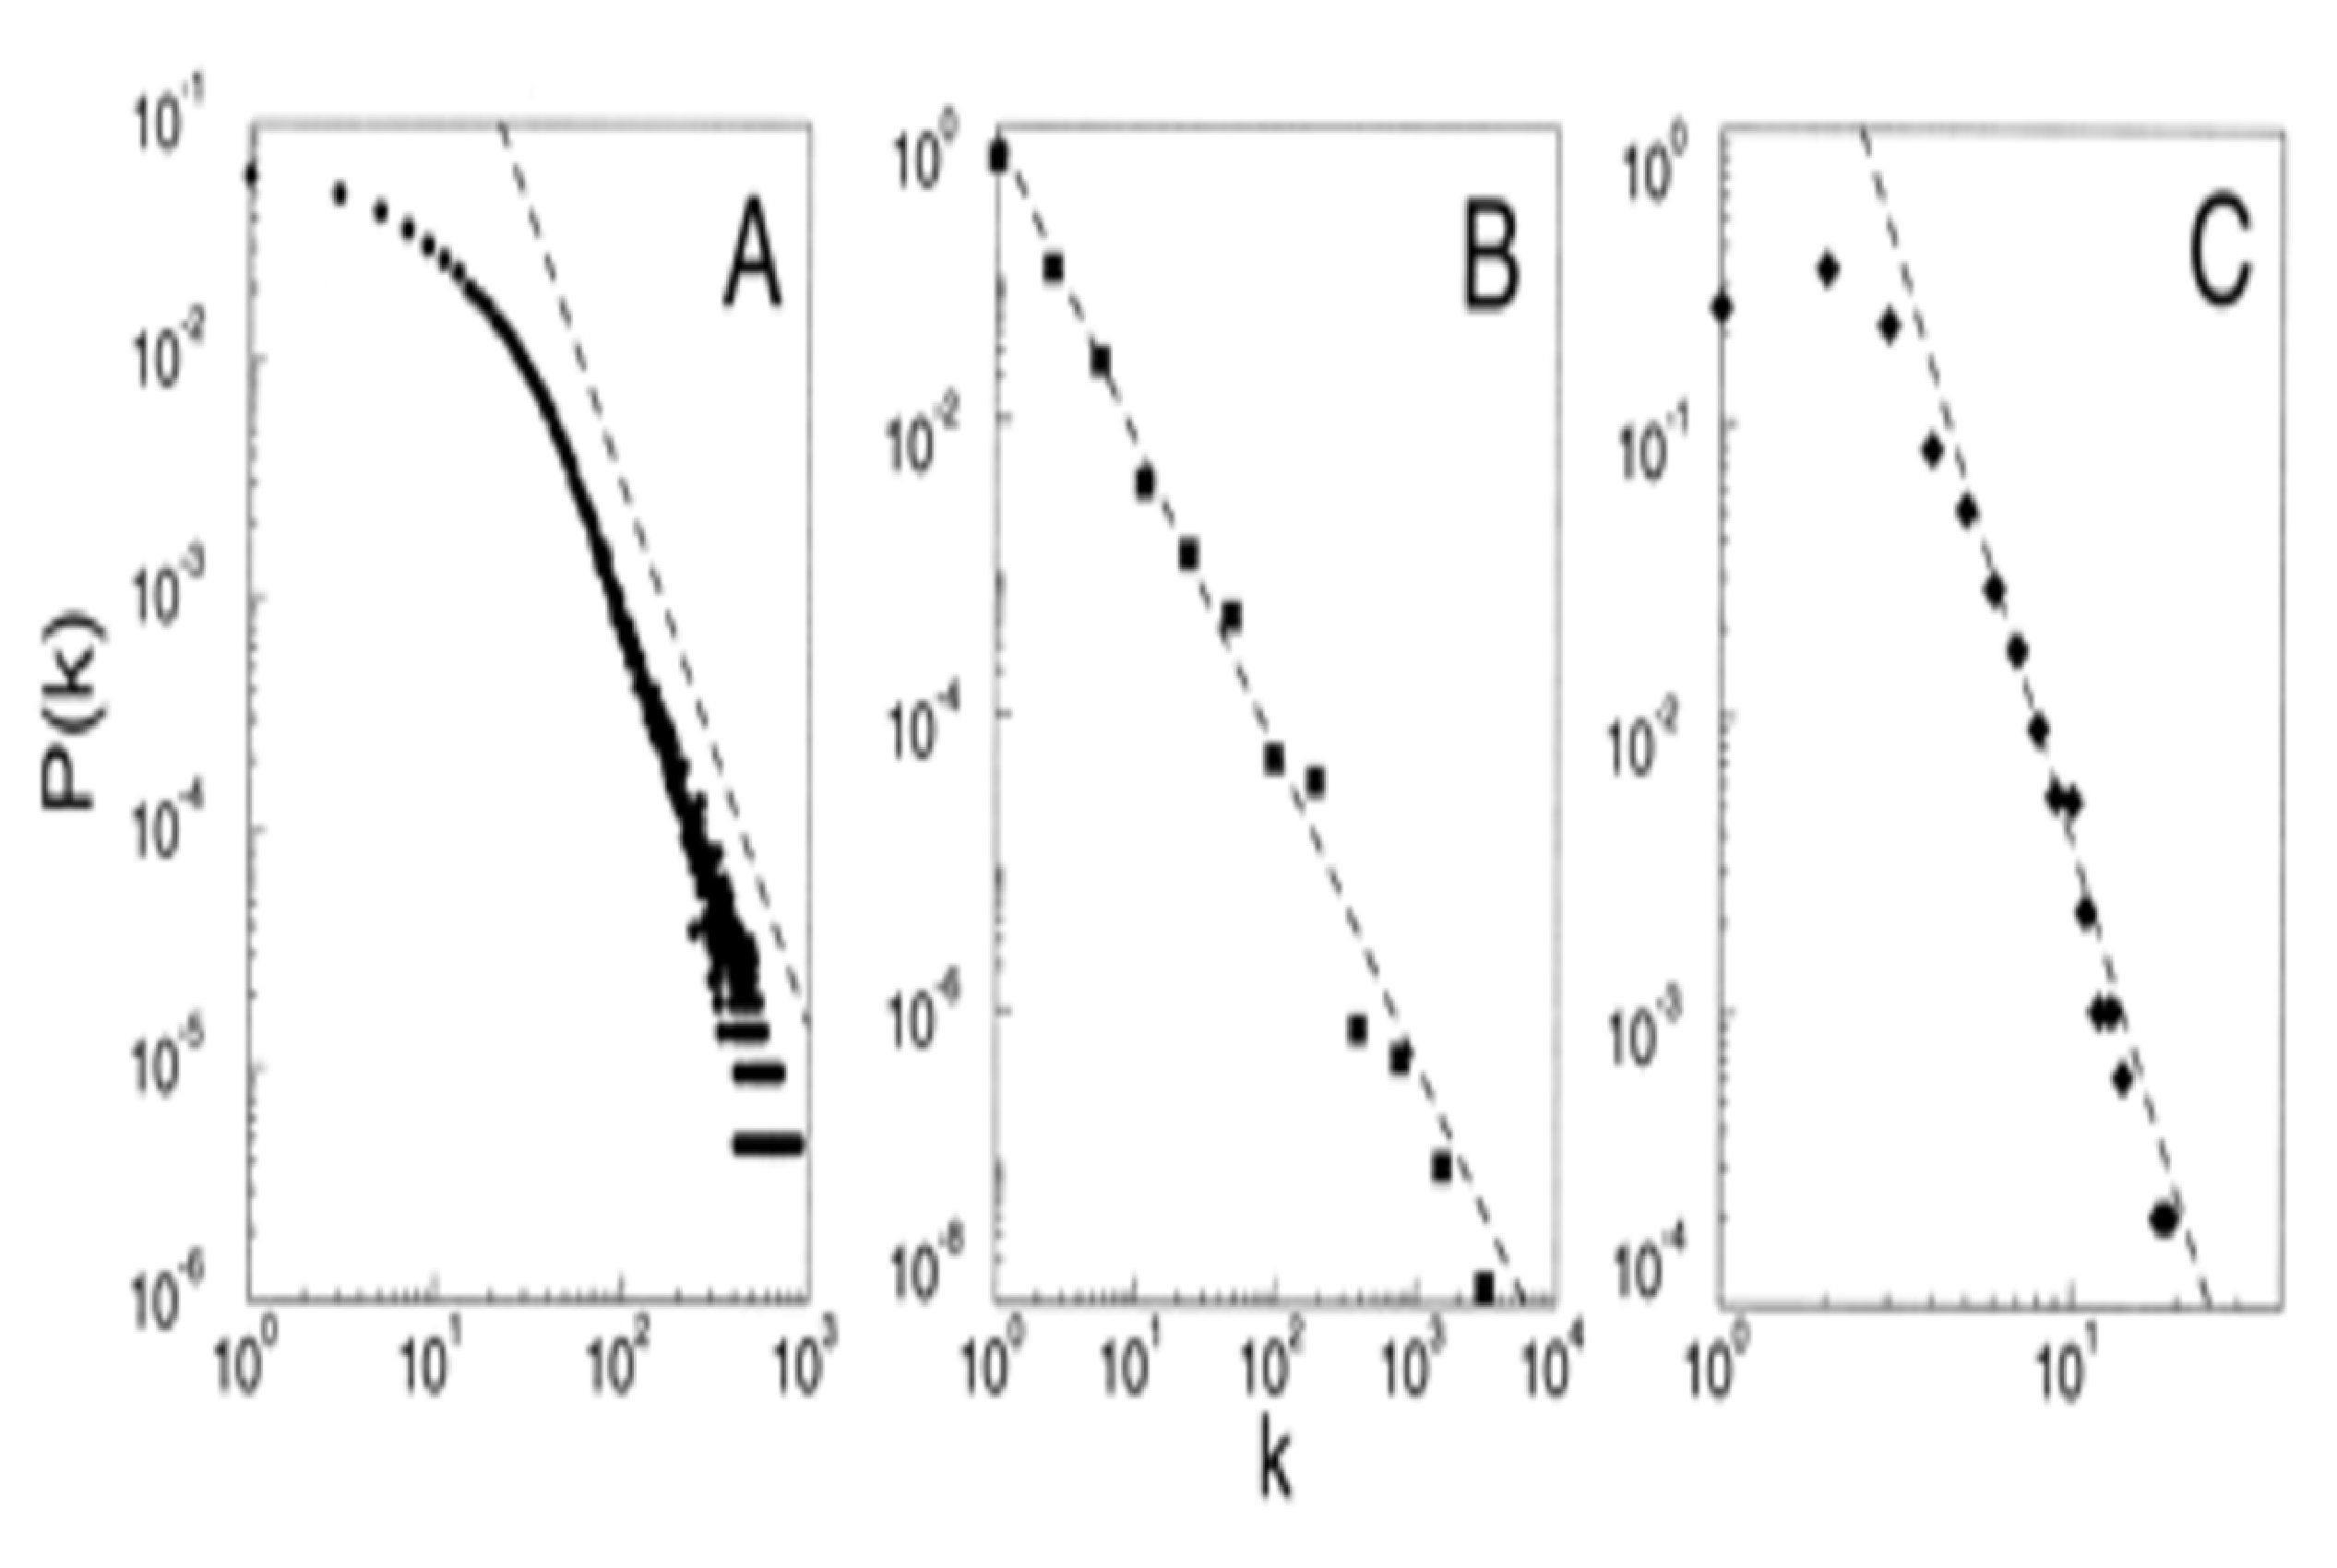
\includegraphics[scale=0.3]{./figures/scal-free-reels}
\caption{Quelques exemples des réseaux sans échelle, (\textbf{A}) Graphe de collaboration d'acteur avec un nombre des nœuds
$n=212250$ et un degré moyen $\textless k\textgreater=28.78$, (\textbf{B}) WWW, $n=325729$, $\textless k\textgreater=5.46$,
(\textbf{C}) Données du réseau électrique, $n=4941$ et $\textless k\textgreater=2.69$. Les lignes pointillées ont des pentes
(\textbf{A}) $\gamma_{actor}=2.3$, (\textbf{B}) $\gamma_{www}=2.1$ et (\textbf{C}) $\gamma_{electrique}=4$.}

\label{scal-free-reels}
\end{figure}
Les distributions de la loi de puissance se produisent dans une gamme de réseaux extraordinairement diversifiée, tels que, les populations des  villes \cite{New2005,Aa-al2009}, la taille des tremblements de terre \cite{GuR1944}, des cratères de la lune  \cite{NeI1994}, la fréquence d'utilisation des mots dans n'importe quelle langue humaine \cite{Zipf1949,Estoup1916}, la  fréquence de l'apparition de noms personnels dans la plupart des cultures \cite{ZaM2001}, le nombre de documents scientifiques écrits \cite{LoW1926}, le nombre de citations reçues par les documents \cite{Price1965}, le nombre de visites sur les pages Web \cite{AdH2000}, les ventes de livres, les enregistrements musicaux et presque tous les autres produits de marque \cite{Cox-al1995}, le nombre d'espèces dans les genres biologiques \cite{WilY1922}, les revenus annuels des personnes \cite{Pareto1896}, les collecteurs de réseaux quantiques complexes \cite{BiR2015} et une foule d'autres réseaux suivent toutes des distributions de loi de puissances.\\

Mathématiquement, une quantité $x$ obéit à une loi de puissance s'elle est tirée d'une distribution de probabilité
\begin{equation}
 P(x)\propto x^{-\gamma}
\end{equation}
Avec $\gamma$ est un paramètre constant de la distribution connue sous le nom d'exposant, empiriquement cet exposant se situe
généralement dans l'intervalle $2<\gamma<3$, bien qu'il existe des exceptions occasionnelles.

\subsection{Structure communautaire}
La société offre une grande variété d'organisations de groupes possibles: les familles, les milieux de travail et d'amitié, les villages, les villes, les nations (voir un exemple dans la Fig.~\ref{community-network}). La diffusion d'Internet a également conduit à la création de groupes virtuels directement sur le Web. Ces communautés se forment également dans de nombreux systèmes en réseau, de la biologie, de l'informatique, de l'ingénierie, de l'économie, de la politique, etc. Par exemple dans le graphe du World Wide Web les communautés peuvent correspondre à des groupes de pages portant sur les mêmes sujets ou des sujets connexes \cite{Dou-al2007,Flak-al2002}. Dans les réseaux d'interactions protéines-protéines, les communautés sont susceptibles de regrouper des protéines ayant la même fonction spécifique dans la cellule \cite{ChY2006,RivT2003}.\\

\begin{figure}[h!]
	\centering
	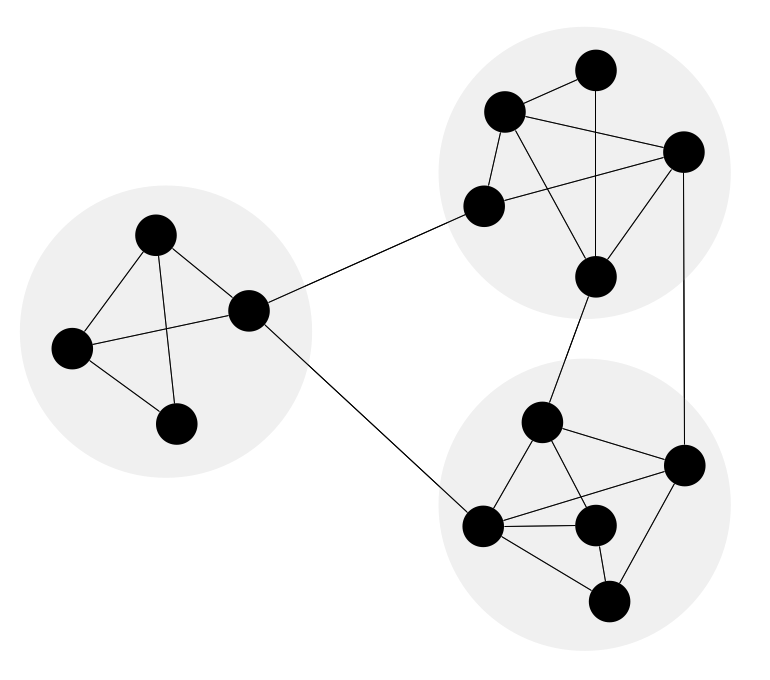
\includegraphics[scale=0.25]{./figures/Network-Community-structure2}
	\caption{Exemples d'un réseau communautaire, on voit trois groupes où chacun est plus connecté par rapport au reste du réseau.}
	\label{community-network}
\end{figure}

Les communautés peuvent avoir des applications concrètes. Le Clustering des clients Web,     qui ont des intérêts similaires et qui sont géographiquement proches les uns des autres, peut améliorer la performance des services fournis sur le WWW, en ce sens chaque groupe de clients pourrait être servi par un serveur miroir dédié \cite{KriW2000}.
Les réseaux auto-configurés formés par des nœuds de communication agissant dans la même région et changeant rapidement, ils n'ont généralement pas de tables de routage centralisées qui spécifient comment les nœuds doivent communiquer entre eux.
Dans ce cas, le regroupement des nœuds en clusters permet de générer des tables de routage compactes, et rend le choix des chemins de communication plus efficace \cite{Steen2001}.\\
La détection communautaire est également importante pour d'autres raisons. L'identification des modules et de leurs limites permet une classification des nœuds, en fonction de leur position structurelle dans les modules. Donc, les nœuds avec une position centrale dans leurs grappes partagent un grand nombre des liens avec les autres partenaires du groupe, ce qui est une caractéristique importante de contrôle et de stabilité au sein du groupe, en outre, Les nœuds situés aux frontières entre les modules jouent un rôle important de médiation et mènent les relations et les échanges entre les différentes communautés \cite{Csermely2008}.

\section{Les modèles théoriques les plus connus} 
Dans cette section, nous citons les modèles théoriques les plus connus et les plus étudiés, en se limitant principalement à des réseaux non pondérés et non orientés, cependant, la plupart des réseaux présentés peuvent être généralisés facilement. Ces modèles se caractérisent chacun par la manière dont les réseaux sont crées et par plusieurs statistiques résultantes, telles que la distribution des degrés, le plus court chemin entre les nœuds et le coefficient de Clustering.

\subsubsection{Réseaux simples}
Un réseau simple consiste en des connexions régulières entre les nœuds. L'un des exemples les plus exceptionnel est le réseau à deux dimensions, comme le montre la Fig.~\ref{Ising2}. Ici, chaque nœud est connecté à ses voisins les plus proches. Malgré sa simplicité, de tels réseaux ont été largement utilisés, par exemple en physique, pour étudier des phénomènes tels que le ferromagnétisme avec le modèle d'Ising \cite{Chowdhury-Stauffer2000}. D'autres exemples de cette classe sont les chaînes linéaires ou les réseaux non rectangulaires tels qu'utilisés, par exemple, dans le contexte de la prédiction de la structure des protéines pour modéliser le repliement de celles-ci \cite{Hsu-al2003,Dehmer2011}.
\begin{figure}[h!]
	\centering
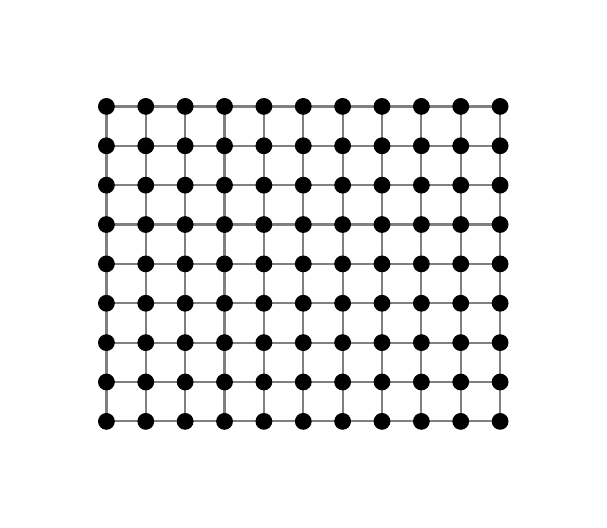
\begin{tikzpicture}
\clip (-1,-1) rectangle (6cm,5cm); 
\draw[style=help lines,thick] (0,0) grid[step=.5cm] (5,4);

\foreach \x in {0,1,...,10}
{
	\foreach \y in {0,1,...,8}
	{
		\node[draw,circle,inner sep=2pt,fill] at (.5*\x,.5*\y) {};
	}
}
\end{tikzpicture}
\caption{Simple réseau régulier de deux dimensions}
\label{Ising2}
\end{figure}
\subsubsection{Réseaux aléatoires}
Les réseaux aléatoires ont été largement étudiés par Erdös et Rényi (ER) \cite{Erdos-Renyi1959,Erdos-Renyi1960,Erdos-Renyi1961}.
Un graphe aléatoire avec $n$ nœuds est obtenu en connectant chaque paire de nœuds avec la probabilité $p$. Le nombre attendu d'arêtes pour un réseau (non orienté) construit
de cette façon est $E=p\frac{n(n-1)}{2}$.
\subsubsection{Réseaux petit-monde}
Mathématiquement, l'effet de petit-monde décrit les graphes dont le diamètre et la longueur moyenne de la trajectoire croissent beaucoup plus lentement que le nombre de nœuds $n$, typiquement en tant que $\ln n$, comme dans un graphe aléatoire ER. Pourtant, un graphe aléatoire a une très faible interconnexion locale, c'est-à-dire le coefficient de regroupement. Watts et Strogatz \cite{Watss-Strogatz1998} ont réalisé un modèle qui rejoint la propriété petit-monde et ayant un coefficient de regroupement fort. Le modèle commence par placer tous les nœuds en cercle, puis connecter chaque nœud à ses premiers $k$ voisins les plus proches, et  avec une probabilité $p$ en prend chaque lien du réseau et on le reconnecte aléatoirement entre deux autres nœuds.
\subsubsection{Réseaux sans échelle}
Ni les réseaux aléatoires ni les réseaux petit-monde ont la propriété sans échelle des degrés, qui est fréquemment
observée dans les réseaux du monde réel. Pour expliquer cette caractéristique, Barab\'{a}si et Albert ont introduit 
un modèle maintenant connu sous le nom de Barab\'{a}si-Albert (BA) \cite{BA1999} ou modèle d'attachement préférentiel
qui aboutit à des réseaux sans échelle qui sont représentés par une distribution des degrés en loi de puissance, 
$P(k)\sim k^{-\gamma}$. La différence majeure entre le modèle d'attachement préférentiel et les autres algorithmes 
décrits ci-dessus pour générer des réseaux aléatoires ou de petit-monde, est que le modèle d'attachement préférentiel
ne suppose pas un nombre fixe de nœuds $n$. Dans ce cas, le réseau croit en ajoutant à chaque instant un noeud qui se connecte aux noeuds dèjà existants avec la probabilité d'attachement préferentielle.

\section{Recours à la physique statistique}
Tous les systèmes mentionnés ci-dessus partagent certaines caractéristiques clés qui les rendent semblables
et appartiennent à la classe des réseaux complexes. On s'intérésse à  comment les 
relations entre les nombreux composants de ces systèmes donnent lieu à des phénomènes ou des comportements 
exprimés par le système dans son ensemble, et non par ses éléments uniques. Ceci indique clairement que
la mécanique statistique est un candidat idéal pour l'investigation et la modélisation de tels systèmes. 
Le but de cette branche de la physique est de décrire l'émergence de certaines propriétés macroscopiques
à partir de la description des interactions des nombreux constituants microscopiques. 
Bien que généralement, dans  les relations des système complexes entre les agents
n'ont pas besoin d'être microscopique, nous pouvons toujours penser que ces interactions sont sur une échelle 
différente (plus petite) par rapport à l'échelle des phénomènes qui émergent du système dans son ensemble, et donc 
la physique statistique peut être utilisée comme un outil puissant pour étudier et dégager les propriétés émergentes 
pertinentes.\\
L'attribut complexe ne signifie pas nécessairement que ces types de systèmes sont compliqués. Cette distinction est
cruciale car les caractéristiques et le comportement des systèmes complexes peuvent différer sensiblement de ceux des 
systèmes compliqués. Différentes branches de la science définissent la complexité de différentes manières selon ce
qui correspond le mieux aux objectifs de leur recherche \cite{NR1998,MMW1993,RG1996,MMAM2009}. Pour cette raison, il n'y a pas d'accord unique sur
cette terminologie et pour ce qui concerne les systèmes complexes, nous citons ici la définition de Neil Johnson sur 
la science complexe comme ``l'étude des phénomènes qui émergent d'une collection d'objets en interaction`` \cite{NFJ2007}.

\let\cleardoublepage\clearpage

